\documentclass[conference]{IEEEtran}
\usepackage[utf8]{inputenc}
\usepackage{listings}
\usepackage{graphicx}
\usepackage[nottoc]{tocbibind}


\usepackage{color}

\lstset{frame=none,
  language=Ruby,
  aboveskip=3mm,
  belowskip=3mm,
  showstringspaces=false,
  columns=flexible,
  basicstyle={\small\ttfamily},
  numbers=none,
  breaklines=true,
  breakatwhitespace=true,
  tabsize=2
}

\begin{document}
\title{Automated Type Contracts Generation in Ruby}
\author
{
    \IEEEauthorblockN
    {
        Nickolay Viuginov 
    }
    
    \IEEEauthorblockA
    {
        Software engineer chairs\\
        St.-Petersburg State University\\
        St.-Petersburg, Russia\\
        Email: viuginov.nickolay@gmail.com
    }
    \and
    \IEEEauthorblockN
    {
        Valentin Fondaratov 
    }
    
    \IEEEauthorblockA
    {
        Team Lead in RubyMine\\
        JetBrains\\
        St.-Petersburg, Russia\\
        Email: fondarat@gmail.com
    }

}
\maketitle

\begin{abstract}
Elegant syntax of Ruby language pays back when it comes to finding bugs in large codebases. Static analysis is
  hindered\cite{ruby_type_checker} by specific capabilities of Ruby, such as defining methods dynamically and evaluating
  string expressions.  Even in dynamically typed languages, type information is very useful, because of better type
  safety and more reliable checks.  One may annotate the code with YARD (Ruby documentation tool) which also enables
  improved tooling such as code completion.

This paper reports a new approach to type annotations generation. We trace direct method calls while the program is
  running, evaluate types of input and output variables and use this information to derive implicit type annotations.

Each method or function is associated with a finite-state automaton, to which all variants of typed signatures are
  added. Then an effective compression technique is applied to the automaton, which reduces the cost of storage and
  allows to display the collected information in a human-readable form.
 
\end{abstract}

\begin{IEEEkeywords}
Ruby, Dynamically typed languages, Ruby VM, YARV, Method signature, Type inference, Static code analysis.
\end{IEEEkeywords}
\IEEEpeerreviewmaketitle

\section{Introduction}
Developers suffer from time-consuming investigations with a goal to understand why the particular piece of code does not
work as expected. The dynamic nature of Ruby allows for great possibilities which has a drawback — the codebase as a
whole becomes entangled and investigations become more difficult compared to the statically typed languages like Java or
C++. Another downside of its dynamic features is a drastic static analysis performance reduction due to inability to
resolve some symbols reliably. 

Consider the dynamic method creation which is often done with \texttt{define\_method} call.  Names and bodies of
dynamically created methods may be calculated at runtime\cite{gradual_type}.
\begin{lstlisting}[
basicstyle=\fontsize{8}{10}\ttfamily,
]
 class User
    ACTIVE = 0
    INACTIVE = 1
    PENDING = 2

    attr_accessor :status

    def self.states(*args)
      args.each do |arg|
        define_method "#{arg}?" do
          self.status == User.const_get(arg.upcase)
        end
      end
    end
    states :active, :inactive, :pending
  end
\end{lstlisting}

One of the possible workarounds is using code documentation tools like RDoc or YARD. % todo cite
As \texttt{@param} and \texttt{@return} annotations may help, they have several drawbacks, too:

\begin{itemize}  
\item the type system used for documenting attributes, parameters and return values is pretty decent however it is not
  clear how to connect the types with each other. For example, \texttt{def []=} for array usually returns the same type
    as the second arg taking any type so in YARD this will look like \texttt{@param~value~[Object]},
    \texttt{@return~[Object]} which is not really helpful.
\item from some perspective, such documentation itself a kind of contradicts the purpose of Ruby — to be as short,
  natural and expressive as possible. 
\end{itemize}

The proposed approach is inspired by the way people tackle this problem manually: one may run or debug the program to
inspect some valuable info about the code they're interested in. This suggests that collecting direct input and output
types of the method dispatches during the program execution, post-processing and structuring of this data will make up
implicit type annotations. As the process is automated, one can retrieve a plenty of information about the covered code.

The collected information not only might be used for YARD annotations generation but also could be stored in a public
database to be shared and reused by different users in order to maximize the coverage of the analyzed code and the
quality of the results. Moreover, generated implicit annotations can be built into the static analysis
tools\cite{Control_flow_analysis_in_scheme}) to improve existing and provide additional checks and code completion
suggestions.

The project implementation can be divided into two main parts:
\begin{itemize}  
  \item At the first stage, the information about called methods and their input and output types is being collected
    thoughout the script execution. It is very important to collect the necessary information as quickly as possible not
    to force users to wait for script completion many times longer compared to the case of the regular execution. To
    achieve this we implement a native extension, which receives all the necessary information directly from the
    internal stack of the virtual machine instead of using the standard API provided by language.

  \item At the second stage, the data obtained in the first stage is structured, reduced to a finite-state automaton and
    prepared for further use in code insight. This storage scheme was chosen because of the ability to quickly obtain a
    regular expression that is easily perceived by a human.
\end{itemize}

\section{Collecting information about method calls}
Method parameters in Ruby have the following structure:
\begin{lstlisting}[
basicstyle=\fontsize{8}{10}\ttfamily,
]
def m(a1, a2, ..., aM,          # mandatory(req)
      b1=(...), ..., bN=(...),  # optional(opt)
      *c,                       # rest
      d1, d2, ..., dO,          # post
      e1:(...), ..., eK:(...),  # keyword
      **f,                      # keyword_rest
      &g)                       # block
\end{lstlisting}


TracePoint is a API allowing to hook several Ruby VM events like method calls and returns and get any data through
Binding, which encapsulates the execution context(variables, methods) and retain this context for future use.
\begin{lstlisting}[
basicstyle=\fontsize{8}{10}\ttfamily,
]

def foo(a, b = 1)
  b = '1'
end

TracePoint.trace(:call, :return) do |tp|
  binding = tp.binding
  method = tp.defined_class.method(tp.method_id)
  p method.parameters
  puts tp.event, (binding.local_variables.map do |v|
    "#{v}->#{binding.local_variable_get(v).inspect}"
  end.join ', ')
end

foo(2)
\end{lstlisting}
\begin{lstlisting}[
basicstyle=\fontsize{8}{10}\ttfamily,
]
[[:req, :a], [:opt, :b]]
call
a->2, b->1
[[:req, :a], [:opt, :b]]
return
a->2, b->"1"
\end{lstlisting}
The big disadvantage of this approach is that calculation of full execution context is a time-consuming operation. But
later we will need information only about a small part of it. Namely: types of arguments, types and names of method
parameters. Creating a native extension for the Ruby VM\cite{Ruby_Under_a_Microscope}, which will receive information
about the method name directly from YARV instruction list (Figure 1) and receive information about argument types
directly from the internal stack. 
\begin{figure}[h]
    \centering
    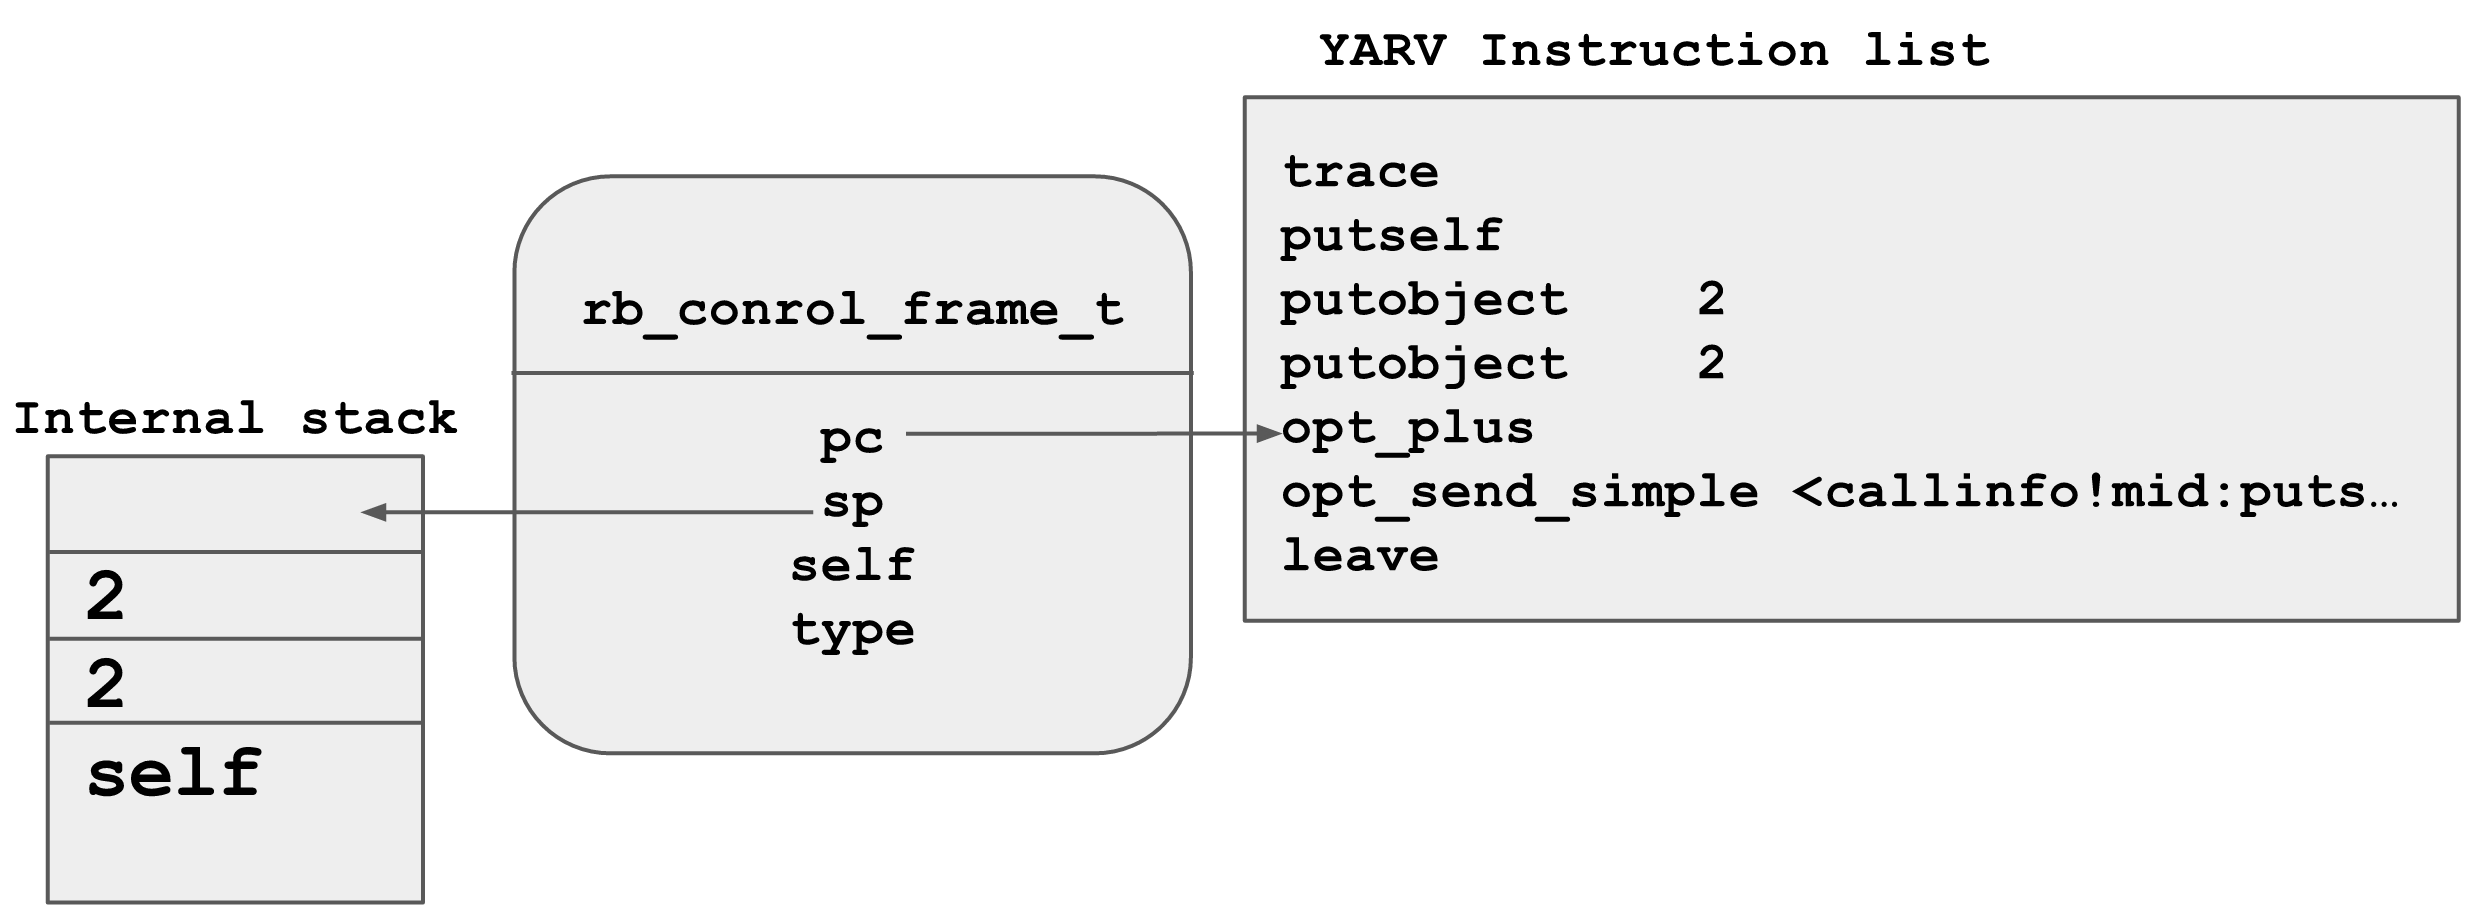
\includegraphics[width=0.5\textwidth]{img1}
    \caption{YARV’s internal registers.}
\end{figure}
Code analysis often handles direct method calls, so it is important to separate which arguments were directly passed to
the method by the user, and which ones were assigned the default values. When Ruby VM hook the call event, all not
specified optional arguments already initialized with default values. So we need to build one more native extension and
gem this information from internal stack. Lets take a look at simple Ruby method with optional parameter and on
appropriate bytecode.
\newpage

\begin{lstlisting}
def foo(a, b=42, kw1: 1, kw2:, kw3: 3)
    #...
end
 
foo(1, kw1: '1', kw2: '2')
\end{lstlisting}
\begin{lstlisting}[
basicstyle=\fontsize{8}{10}\ttfamily,
]
== disasm: #<ISeq:<compiled>@<compiled>>============
0000 trace            1
0002 putspecialobject 1
0004 putobject        :foo
0006 putiseq          foo
0008 opt_send_without_block <callinfo!mid:core#define_method, argc:2, ARGS_SIMPLE>
0011 pop
0012 trace            1                                               
0014 putself          
0015 putobject_OP_INT2FIX_O_1_C_ 
0016 putstring        "1"
0018 putstring        "2"
0020 opt_send_without_block <callinfo!mid:foo, argc:3, kw:[kw1,kw2], FCALL|KWARG>
0023 leave
== disasm: #<ISeq:foo@<compiled>>===================
0000 putobject        42
0002 setlocal_OP__WC__0 6
0004 trace            8
0006 putnil
0007 trace            16
0009 leave    
\end{lstlisting}
So we need to find bytecode instruction for current method dispatch. For this, it is necessary to find caller control
frame, and get last executed instruction in this frame. Thats how we get number of arguments(argc:) and list of key
words(kw:[])
\section{Transforming raw call data into contracts}
Huge amount of raw signatures received from the Ruby process must be structured and processed so that it can be easily
used and perceived. Each traced method is associated with a finite-state automaton. This storage structure allows you to
quickly add raw data obtained from the Ruby process. It is also can easily be reduced to a human-readable regular
expression. 
\begin{figure}[h]
    \centering
    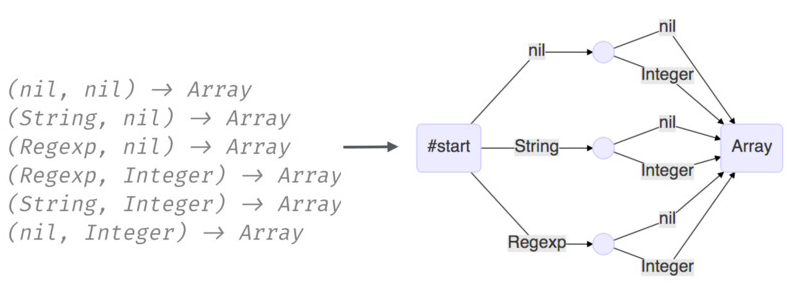
\includegraphics[width=0.42\textwidth]{img2}
    \caption{Example of generating a non-minimized automaton.}
\end{figure}
\newpage
In each automaton there is a single starting vertex and a single terminal vertex. To the automaton consistently added
words obtained by concatenating signatures and corresponding output types. Then the minimization
algorithm\cite{dfa_minimisation} is applied to this automaton. Quite often there are situations when the types of the
two or more arguments of the method always coincide. Or even the type of the result coincides with type of one of the
arguments. Consider an algorithm of processing such methods using method \texttt{equals} as an example.
\begin{lstlisting}[
basicstyle=\fontsize{8}{10}\ttfamily,
]
def equals(a, b)
  raise StandardError if a.class != b.class
  a == b
end
p equals(1, 1) # (Integer, Integer) -> TrueClass
p equals(1, 2) # (Integer, Integer) -> FalseClass
...
\end{lstlisting}
\begin{figure}[h]
    \centering
    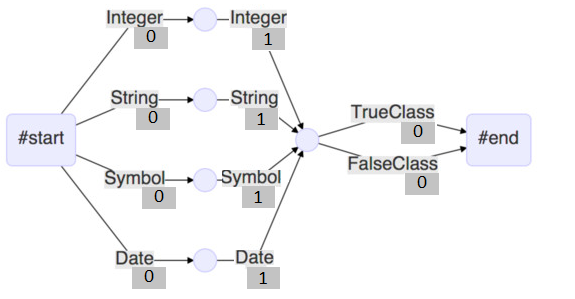
\includegraphics[width=0.4\textwidth]{img4}
    \caption{Automaton with counted bit masks.}
\end{figure}
In this case, the types of arguments are the same, so the automaton can be markedly reduced. The algorithm consists in
storing a bit mask on each automaton transition. Bit with one indicates a match of the type written on the edge with
the corresponding previous type (Fig 3). In case the mask is greater than 0, the type written on the edge can be
replaced with a mask. Subsequently, the transition along the edge will be carried out only when a readable signature is
applied to the mask. After that, minimization algorithm is applied to the automaton one more time.
\begin{figure}[h]
    \centering
    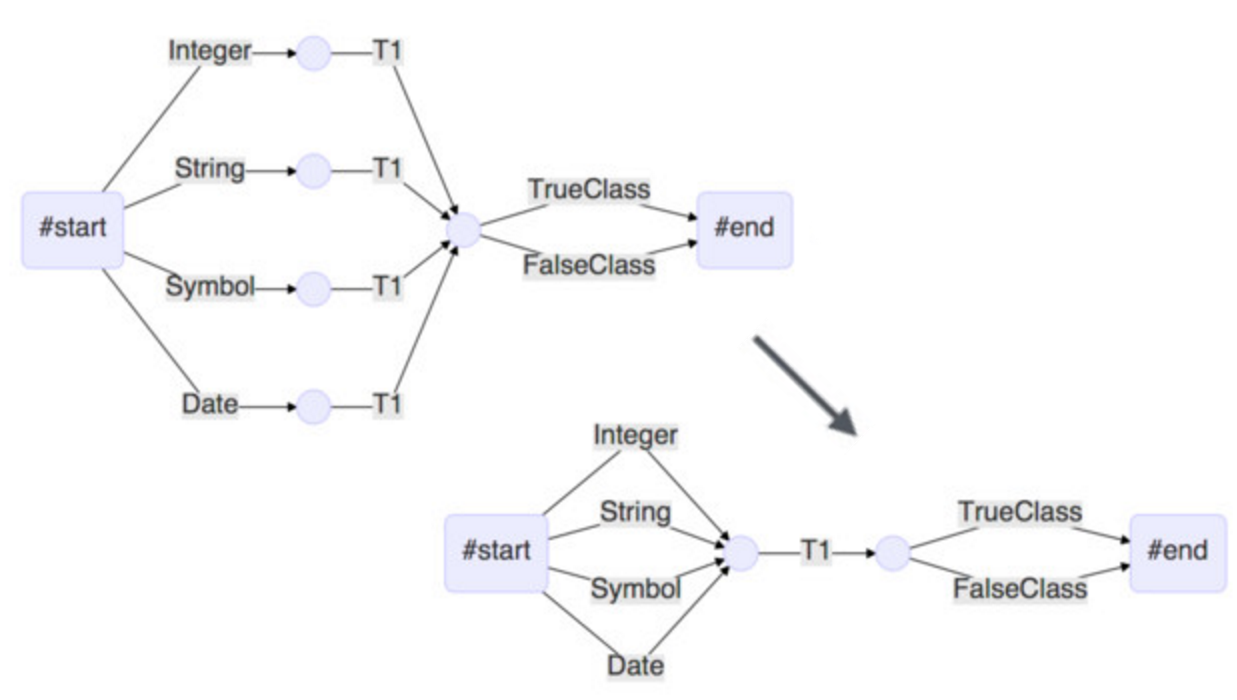
\includegraphics[width=0.5\textwidth]{img5}
    \caption{Minimizing the automaton with reference edges.}
\end{figure}
\\
\\
When during the code analysis it will be necessary to calculate the type returned by the method, we simply read through
the automaton the set of input types of this method, and all the transitions from the vertex in which we turn out to be
the desired output types.
\section{Conclusion}
The paper describes the approach to generation of implicit type annotations.
\par This approach provides information about the types of methods that can not be obtained by static analysis of the source code in case if it is possible to understand in which library the method was declared and resolve the method receiver. This approach is useful for methods that are declared dynamically or in their body there are complex syntactic constructions, for example evaluating a string variable.
\par At the moment, we are working on optimizing
the time of collecting of statistics. In the future, it will be necessary to test the approach, carry out load testing
and implement the prototype in the existing static analysis of the Ruby language.

\bibliographystyle{unsrt}
\bibliography{sample.bib}
\end{document}